\chapter{Methods}

Considering the huge dimension of the dataset and the fact that a large portion of its content was
useless, smaller datasets have been computed with the aim of expediting the analysis even for future
usages. The analysis was made based on the computed datasets. These datasets can be computed for
every language thanks to a bash script, in this way a multilingual analysis on the most
controversial topics can be conducted in different locations.


\bigskip



\tikzstyle{square} = [rectangle, rounded corners, minimum width=3cm, minimum height=1cm,text centered,text width=3cm, draw=black, fill=blue!20]
\tikzstyle{arrow} = [thick,->,>=stealth]

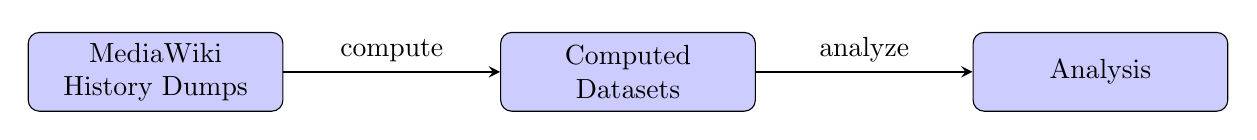
\begin{tikzpicture}[node distance=4cm]
    \node (dataset) [square, xshift=4cm] {MediaWiki History Dumps};
    \node (computed) [square, right of=dataset, xshift=2cm] {Computed Datasets};
    \node (anal) [square, right of=computed, xshift=2cm] {Analysis};

    \draw [arrow] (dataset) --node[anchor=south] {compute}(computed);
    \draw [arrow] (computed) -- node[anchor=south]{analyze}(anal);

\end{tikzpicture}

\bigskip

\section{Computed Dataset}
After the first skimming, only the revisions involving a revert were left. This dataset, whose
schema is the same as the MediaWiki History Dumps, has been sorted by both page and timestamp,the
size is now \~10\% of the originaland thanks to this screening. To achieve this we went through the
compressed dataset line by line decompressing it on the fly and saving in a file only the entries we
were interested in. Due to this the amount of ram required is very small and so is the disk space
since all data is compressed. For the sorting part, we used Unix sort, which is the most optimized
way to sort a file like this.  

From this filtered dataset have been computed several smaller datasets which can be divided into two modules: 

\begin{itemize}
    \item Chains: in these datasets, the focus was on detecting revert chains in pages 
    \item Group: in these datasets, the focus was on the number of reverts that users did or received based on the groups ( admin, registered, anonymous).
\end{itemize}

\subsection{Chains}
The data about revert chains were computed from the compressed filtered dataset. Every time we used
the filtered dataset we read it line by line, saving only the interesting information. The output
is a JSON file, where each page corresponds a JSON object. For each page we save the list of chains
and some statistics. A chain has a start and an end date, a list of revisions, and the users
involved. This dataset is way smaller than the initial one so it is possible to browse the dataset
in few seconds.\\


To identify a chain we used a function called \textit{simple\_chains} that differs from another called
\textit{complex\_chains} for the fact that the first one to identify a chain of revert considers only
contiguous reverts. We decided to use the simple one because we are only interested in chains that
occur in a short time span since that is where most of the discussions take place. If more than
50\% of users involved in a chain are bots the chain is not saved. There are two versions of this
dataset, one that considers anonymous users and one that does not. \\

In the schema below there are all the fields in a page object. 
\begin{verbatim}
    {
        "title": "Loligo_vulgaris", 
        "chains": 
        [{
            "revisions": ["113715375", "113715381", "113715393"], 
            "users": {"62.18.117.244": "", "Leo0428": "17181"}, 
            "len": 3, 
            "start": "2020-06-15 22:16:23.0", 
            "end": "2020-06-15 22:17:38.0"
        }], 
        "n_chains": 1, 
        "n_reverts_in_chains": 3, 
        "n_reverts": 38
        "mean": 3.0, 
        "longest": 3, 
        "G": 0,
        "M": 0, 
        "lengths": {"3": 1}
    }
    
\end{verbatim}


Regarding users, the object is very similar, but it is calculated differently. All the data we need
is stored in the JSON pages. By analyzing that file you can extract all the chains in which a user
has been involved and then calculate statistics in a similar way as for pages. Using this dataset
allow us to compute this dataset 10 times faster.  

The only difference is that the M field is missing because it is only related to a page. The field G, instead,
can be computed on a user considering every chain where it is the author of at least a revision.\\

The dataset was also calculated monthly for both users and pages, the schema is simpler than the
JSON and this allows us to save it in a TSV using only one row for each month. Instead of saving
all the data about the chain, we save the number of chains that are longer than 5,7,9. In Table
\ref{table:chainsPagemonth} there is a sample page entry. To do this we have processed the
JSON database one page (or user) at a time by dividing by month. We counted the chains per month basing
on the start date of the chain.   

\begin{table}[H]
    \centering
    \ra{1.2}
    \begin{tabularx}{\columnwidth}{@{}Xcccccccccc@{}}
        \midrule
        \textbf{title} & \textbf{year\_month} & \textbf{nchain} & \textbf{nrev} & \textbf{mean} & \textbf{longest} & \textbf{$\geq$ 5} & \textbf{$\geq$ 7} & \textbf{$\geq$ 9} & \textbf{G}\\ \toprule
        Loligo\_vulgaris & 2020-10 & 1 & 15 & 3.0 & 3 & 0 & 0 & 0 & 0\\
        
        \bottomrule
    \end{tabularx}
    
    \caption{entry of the mothly tsv \label{table:chainsPagemonth}}
\end{table}


\subsection{Group}
Another interesting part of the study was focusing on the category a user belongs. Thanks to this we
are able to track the habits of the users allowing us to understand, for example, if someone stops
editing Wikipedia after several reverts from admins. Detecting these kinds of patterns is useful for
community health: a user can be warned if its behavior could lead to a drop-off. The groups to which
users can belong are: 


\begin{itemize}
    \item Admin (sysop): can perform certain actions like blocking users and editing protected pages, 
    \item Registered: are logged in at the time of the edit, 
    \item Anonymous: are not logged in and their username is their IP address(it is not possible to match an IP with a user
        because the IP can change over time).
\end{itemize}

The datasets computed are both for pages and users: 
\paragraph*{Pages} 
For each page, there are two topics of investigation: reverts and mutual reverts. An entry of the
dataset is a page-month and gives us the number of reverts and mutual reverts made on the page
divided by group. This can be helpful, for example, to detect pages where admins are more active and
this could be a sign that something is wrong with the page.



The notation \textit{adm\_reg} in Table \ref{table:revertpage} refers to the number of admin that performed a
revert to a registered user (similarly with \textit{adm\_adm, reg\_adm, reg\_reg} ).\\

The notation \textit{mut\_ra} in the Table \ref{table:mutualpage} refers to the number of mutual reverts
where the users involved are a registered one and an admin, the order does not matter, in fact, there is
no \textit{mut\_ar} that would have the same value.\\


Since the focus was on experienced users, only pairs involving registered and admins were computed.
For having an idea of the volume of the reverts made by anon we saved the number of reverts
that were made by both anonymous (\textit{anon}) and not anonymous (\textit{not\_anon}).

To calculate these metrics we use simple variables that are incremented as you scroll through the filtered dataset
and initialized each time a new page is started. For both users and pages, we have discarded
edits that have been marked as vandalism and edits made by bots.

\begin{table}[H]
    \centering
    \ra{1.2}
    \begin{tabularx}{\columnwidth}{@{}Xcccccccccc@{}}
        \midrule
        \textbf{id} & \textbf{page} & \textbf{year\_month} & \textbf{adm\_adm} & \textbf{adm\_reg} & \textbf{reg\_adm} & \textbf{reg\_reg} & \textbf{anon} & \textbf{not\_anon}\\ \toprule
        1 & pagina & 2020-10 & 13 & 12 & 42 & 0 & 0 & 0 \\
        
         \bottomrule
    \end{tabularx}
    
    \caption{entry of the revert page tsv \label{table:revertpage}}
\end{table}

In the case of mutual reverts the procedure is similar but a bit more complex because we need to
store the information of the whole page in order to correctly detect all the mutual reverts. 
The most efficient way to save such information is the use of dictionaries where we saved for each
reverter the list of users who reverted and then at page processing time we computed a list of pairs
that were used to calculate the other metrics.

\begin{table}[H]
    \centering
    \ra{1.2}
    \begin{tabularx}{\columnwidth}{@{}Xcccccccccc@{}}
        \midrule
        \textbf{id} & \textbf{page} & \textbf{year\_month} & \textbf{mut\_aa} & \textbf{mut\_ra}  & \textbf{mut\_rr} & \textbf{anon} & \textbf{not\_anon}\\ \toprule
        1 & pagina & 2020-10 & 13 & 12 & 42  & 0 & 0 \\
         \bottomrule
    \end{tabularx}
    
    \caption{entry of the mutual page TSV \label{table:mutualpage}}
\end{table}

\paragraph*{User}
It is useful also to have the data aggregated by user. Reverts data can be retrieved from the
filtered dataset sorted by timestamp. The data about reverts is gathered and processed month by
month, this allowed us to save for each user-month the number of reverts made and received divided
by group.

In this case, the dataset is browsed and processed month by month. When a user performs a revert the
dataset gives us the id of the revision it has reverted but not the id of the user it has
reverted. To solve this problem so we had to save the info in different dictionaries: \textit{reverters, editor, groups}, 
\bigskip

reverters[username] gives us the list of the revision it reverted. \\
\indent editor[revision\_id] gives us the user who performs that edit. \\
\indent groups[username] gives us the groups a user belongs.\\


Combining this dictionaties we have all the data necessary to compute all the metrics we need.
\begin{table}[H]
    \centering
    \ra{1.2}
    \begin{tabularx}{\columnwidth}{@{}ccc@{}}
        \midrule
        \textbf{user} & \textbf{group} & \textbf{year\_month} \\ \toprule
        carlos & adm & 2020-10  \\
        
         \bottomrule
    \end{tabularx}
    \begin{tabularx}{\columnwidth}{@{}XXXXXXXX@{}}
        \midrule
        \textbf{received} & \textbf{r\_reg}  & \textbf{r\_not} & \textbf{r\_adm} & \textbf{done} & \textbf{d\_reg} & \textbf{d\_not} & \textbf{d\_adm}\\ \toprule
        13 & 12 & 42  & 0 & 13 & 12 & 42  & 0  \\
        
         \bottomrule
    \end{tabularx}
    
    \caption{entry of the mutual page tsv \label{table:revks}}
\end{table}


The mutual revert analysis was more difficult to implement because to save the information about
mutual reverts we need the dataset sorted by pages, but to get the data by user we should use the
one sorted by timestamp. We solved this problem by storing the user-page-month in the dataset, so
the information about the mutual returns of a user involved in a specific month on a specific page.
This led to a larger dataset but with a higher level of information: it is easy to post-process the dataset
by grouping by user or by month to have one entry per user or one entry per month,
respectively. 


\begin{table}[H]
    \centering
    \ra{1.2}
    \begin{tabularx}{\columnwidth}{@{}XXXXXXX@{}}
        \midrule
        \textbf{user} & \textbf{group} & \textbf{page\_name}& \textbf{year\_month} & \textbf{mut\_adm}& \textbf{mut\_reg}& \textbf{mut\_not}\\ \toprule
        khalu & adm & pagina & 2020-10 & 13 & 12 & 4 \\
        
         \bottomrule
    \end{tabularx}

    
    \caption{entry of the mutual page tsv \label{table:rjevks}}
\end{table}







